% gc-12-Fundamental.tex

\documentclass[xcolor=dvipsnames]{beamer}

\usepackage{cancel}
\renewcommand{\CancelColor}{\color{red}}
\usepackage{graphicx}
\usepackage{wrapfig}
\usepackage{colortbl}
\usepackage{color}
\usepackage{alltt}
\definecolor{myblue}{rgb}{0.8,0.85,1}

\mode<presentation>
{
  \usetheme{Warsaw}
  \setbeamercovered{transparent}
}
% \usecolortheme[named=OliveGreen]{structure}
\setbeamertemplate{navigation symbols}{} 
\setbeamertemplate{blocks}[rounded][shadow=true] 

\newcounter{expls}
\setcounter{expls}{0}
\newcommand{\beispiel}[1]{\refstepcounter{expls}\textbf{Example \arabic{expls}: #1.}}

\newcounter{exercise}
\setcounter{exercise}{0}
\newcommand{\ubung}[0]{\refstepcounter{exercise}\textbf{Exercise \arabic{exercise}: }}

\newif\ifBCITCourse
\BCITCoursetrue
% \BCITCoursefalse
\newif\ifWhichCourse
\WhichCoursetrue
\WhichCoursefalse
\ifBCITCourse
\ifWhichCourse
\newcommand{\CourseName}{Statistics for Food Technology}
\newcommand{\CourseNumber}{MATH 2441}
\newcommand{\CourseInst}{BCIT}
\else
\newcommand{\CourseName}{Calculus for Geomatics}
\newcommand{\CourseNumber}{MATH 2511}
\newcommand{\CourseInst}{BCIT}
\fi
\else
\newcommand{\CourseName}{Philosophy and Literature}
\newcommand{\CourseNumber}{PHIL 375}
\newcommand{\CourseInst}{UBC}
\fi

\title{Fundamental Theorem of Calculus}
\subtitle{{\CourseNumber}, BCIT}

\author{\CourseName}

\date{March 6, 2017}

\begin{document}

\begin{frame}
  \titlepage
\end{frame}

\begin{frame}
  \frametitle{Antiderivatives}
Remember these two problems that we wanted to solve when we started
with calculus:
  \begin{figure}[h]
    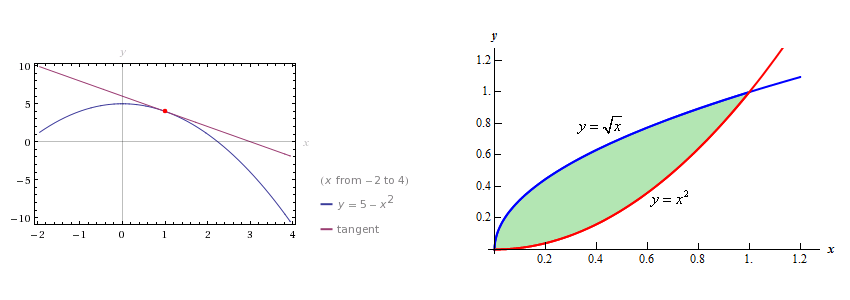
\includegraphics[scale=.35]{./diagrams/regiontangent.png}
  \end{figure}
We have solved the problem on the left. Now it is time to solve the
problem on the right. For areas under a curve, we need
antiderivatives. The antiderivative $F(x)$ of a function $f(x)$ is the
function for which $F'(x)=f(x)$. 
\end{frame}

\begin{frame}
  \frametitle{Differential Equations}
Differential equations are like regular equations except that the
unknown is a function, not a variable. Remember that
\begin{equation}
  \label{eq:aiceiphe}
  dy=f'(x)\,dx\mbox{, therefore }f'(x)=\frac{dy}{dx}
\end{equation}
Now consider this differential equation,
\begin{equation}
  \label{eq:pheiwaot}
  \frac{dy}{dx}=f(x)
\end{equation}
This is an ODE, an \alert{ordinary differential equation}. 
\end{frame}

\begin{frame}
  \frametitle{Differential Equations}
\begin{equation}
  \label{eq:ahngohto}
  \frac{dy}{dx}=f(x)
\end{equation}
This is an ODE, an \alert{ordinary differential equation}. Any
function
\begin{equation}
  \label{eq:ogheigha}
  f(x)=e^{x}+C,C\in\mathbb{R}
\end{equation}
would solve it. Often, an \alert{initial condition} is provided to
make the solution unique. Therefore, the solution to the differential
equation
\begin{equation}
  \label{eq:joogeipo}
  \frac{dy}{dx}=f(x)
\end{equation}
with initial condition $f(0)=1$ is $f(x)=e^{x}$.
\end{frame}

\begin{frame}
  \frametitle{Differential Equations}
Antiderivatives are solutions to special differential equations. For
example, the antiderivative of $f(x)=6x$ is the solution to the
differential equation
\begin{equation}
  \label{eq:xoozazui}
  \frac{dy}{dx}=6x
\end{equation}
With an initial condition, the solution to this equation may be
unique.
\end{frame}

\begin{frame}
  \frametitle{Rules for Finding Antiderivatives}
  Antiderivatives are not unique. If $F(x)$ is an antiderivative for
  $f(x)$, then $F(x)+c$ is an antiderivative as well, where $c$ is any
  real number. In the following, we will use the notation $F(x)$ for
  one arbitrary antiderivative. There are many rules for finding
  antiderivatives called \emph{table of integrals}. Here are a few.
  \begin{block}{Rule 1}
    If you find a function $g(x)$ for which $g'(x)=f(x)$, then
    $F(x)=g(x)+c$.
  \end{block}
  Exercise: show that the function $g(x)$ is an antiderivative of
  $f(x)=(x^{3}+3)^{6}(3x^{2})$.
  \begin{equation}
    \label{eq:eiyahcei}
    g(x)=\frac{(x^{3}+3)^{7}}{7}
  \end{equation}
\end{frame}

\begin{frame}
  \frametitle{More Rules for Finding Antiderivatives I}
  \begin{block}{Rule 2}
    If $F(x)$ is an antiderivative for $f(x)$, then $aF(x)$ is an
    antiderivative for $af(x)$, where $a$ is a constant.
  \end{block}
\end{frame}

\begin{frame}
  \frametitle{More Rules for Finding Antiderivatives II}
  \begin{block}{Rule 3}
    If $F_{1}(x)$ is an antiderivative for $f_{1}(x)$ and $F_{2}(x)$
    is an antiderivative for $f_{2}(x)$, then $F_{1}(x)+F_{2}(x)$ is
    an antiderivative for $f_{1}(x)+f_{2}(x)$.
  \end{block}
\end{frame}

\begin{frame}
  \frametitle{More Rules for Finding Antiderivatives III}
  \begin{block}{Rule 4}
    If $f(x)=x^{n}$ and $n\neq{}-1$, then $F(x)=\frac{x^{n+1}}{n+1}$
    is an antiderivative of $f(x)$.
  \end{block}
Exercise: Find an antiderivative of $f(x)=1/x$. The answer is not
quite what you would expect (but very close). 
\end{frame}

\begin{frame}
  \frametitle{Summary}
Here is a table of antiderivatives, where $F$ is an antiderivative of
$f$ and $G$ is an antiderivative of $g$.

\medskip

\begin{tabular}{|l|l|}\hline
  $cf(x)$ & $cF(x)$ \\ \hline
  $f(x)+g(x)$ & $F(x)+G(x)$ \\ \hline
  $x^{n}$ with $n\neq{}-1$ & $\displaystyle \frac{x^{n+1}}{n+1}$ \\ \hline
  $\displaystyle \frac{1}{x}$ & $\ln\vert{}x\vert$ \\ \hline
  $e^{x}$ & $e^{x}$ \\ \hline
  $\cos{}x$ & $\sin{}x$ \\ \hline
  $\sin{}x$ & $-\cos{}x$ \\ \hline
  $\sec^{2}x$ & $\tan{}x$ \\ \hline
  $\sec{}x\tan{}x$ & $\sec{}x$ \\ \hline
  $\displaystyle \frac{1}{\sqrt{1-x^{2}}}$ & $\arcsin{}x$ \\ \hline
  $\displaystyle \frac{1}{1+x^{2}}$ & $\arctan{}x$ \\ \hline
\end{tabular}
\end{frame}

\begin{frame}
  \frametitle{Integration}
  The process of finding a derivative is called differentiation. The
  process of finding an antiderivative is called \alert{integration}.
  Instead of the symbol `prime' ($f'(x)$) for differentiation we use
  the sign $\int$ for integration. The symbol $\int$ stands for the
  word `sum' because we take the limit of a sum of areas in order to
  find the area under a curve.
\begin{equation}
  \label{eq:muixutoh}
  \int{}f(x)\,dx=F(x)+c
\end{equation}
The differential helps to identify which letter is the variable for
the function (there may be other letters that are just constants), for
example
\begin{equation}
  \label{eq:eighooko}
  \int{}ax^{2}\,dx=\frac{ax^{3}}{3}+c
\end{equation}
\begin{equation}
  \label{eq:ungiumah}
  \int{}ax^{2}\,da=\frac{a^{2}x^{2}}{2}+c
\end{equation}
\end{frame}

\begin{frame}
  \frametitle{Integration Exercises I}
Find the following \alert{indefinite integrals} (another expression
for antiderivatives). 
\begin{equation}
  \label{eq:eevoomoh}
  \int{}6\,dx
\end{equation}
\begin{equation}
  \label{eq:eohauthu}
  \int{}-2\,dx
\end{equation}
\begin{equation}
  \label{eq:heizieta}
  \int{}8x^{4}\,dx
\end{equation}
\begin{equation}
  \label{eq:zohjieph}
  \int{}\pi{}x^{3}\,dx
\end{equation}
\begin{equation}
  \label{eq:oodaelad}
  \int{}\left(x^{3}+7-2x^{2}\right)\,dx
\end{equation}
\begin{equation}
  \label{eq:eeshooyo}
  \int{}\sqrt{x}\,dx
\end{equation}
\begin{equation}
  \label{eq:uafievai}
  \int{}\frac{7}{2}x^{\frac{5}{2}}\,dx
\end{equation}
\end{frame}

\begin{frame}
  \frametitle{Integration Exercises II}
Find the following \alert{indefinite integrals} (another expression
for antiderivatives). 
\begin{equation}
  \label{eq:igheivei}
  \int{}9\sqrt[5]{2x}\,dx
\end{equation}
\begin{equation}
  \label{eq:akahheju}
  \int{}\frac{3}{x^{3}}\,dx
\end{equation}
\begin{equation}
  \label{eq:zeifahce}
  \int{}\frac{7}{\sqrt[3]{x}}\,dx
\end{equation}
\begin{equation}
  \label{eq:afahthud}
  \int{}\sqrt{x}\left(3x-2\right)\,dx
\end{equation}
\begin{equation}
  \label{eq:desheiga}
  \int{}\left(x+1\right)^{2}\,dx
\end{equation}
\begin{equation}
  \label{eq:oongaiqu}
  \int{}\frac{4x^{2}-2\sqrt{x}}{x}\,dx
\end{equation}
\begin{equation}
  \label{eq:ahxiequo}
  \int{}\frac{x^{3}+2x^{2}-3x-6}{x+2}\,dx
\end{equation}
\end{frame}

\begin{frame}
  \frametitle{Definite Integrals I}
Evaluating an integral at a point doesn't give us anything
particularly meaningful.
\begin{equation}
  \label{eq:beavaika}
  \int{}x^{2}\,dx=\frac{x^{3}}{3}+c
\end{equation}
\begin{equation}
  \label{eq:paeshohz}
  \left.\int{}x^{2}\,dx\right\vert_{x=6}=\frac{6^{3}}{3}+c=72+c
\end{equation}
However, if we subtract one evaluated integral from another, we get a number.
\begin{equation}
  \label{eq:phiasohm}
  \left.\int{}x^{2}\,dx\right\vert_{x=6}-\left.\int{}x^{2}\,dx\right\vert_{x=3}=\frac{6^{3}}{3}+c-\left(\frac{3^{3}}{3}+c\right)=72-9=63\notag
\end{equation}
\end{frame}

\begin{frame}
  \frametitle{Definite Integrals II}
We call this difference between evaluated integrals \alert{definite
  integral}. The notation is
\begin{equation}
  \label{eq:yooxiefi}
  \int_{3}^{6}x^{2}\,dx=\left.\int{}x^{2}\,dx\right\vert_{x=6}-\left.\int{}x^{2}\,dx\right\vert_{x=3}=63\notag
\end{equation}
\end{frame}

\begin{frame}
  \frametitle{Definite Integrals Exercises}
Evaluate each definite integral.
\begin{equation}
  \label{eq:ufaetohm}
  \int_{1}^{2}x\,dx\hspace{1in}  \int_{-2}^{2}x^{2}\,dx
\end{equation}
\begin{equation}
  \label{eq:vahyooyi}
  \int_{1}^{3}7x^{2}\,dx\hspace{1in}  \int_{-2}^{2}3s^{4}\,ds
\end{equation}
\begin{equation}
  \label{eq:wohbuxoo}
  \int_{0}^{4}(x^{2}+2x)\,dx\hspace{1in}  \int_{1}^{e}\frac{1}{x}\,dx
\end{equation}
\begin{equation}
  \label{eq:ohgooquu}
  \int_{5}^{10}\sqrt{x}\,dx\hspace{1in}\int_{1}^{4}\frac{2+x^{2}}{\sqrt{x}}\,dx
\end{equation}
\begin{equation}
  \label{eq:yoocaitu}
  \int_{-1}^{2}(3u-2)(u+1)\,du\hspace{1in}\int_{\frac{\pi}{6}}^{\pi}\sin\vartheta{}\,d\vartheta
\end{equation}
\end{frame}

\begin{frame}
  \frametitle{Fundamental Theorem of Calculus I}
  It turns out that the definite integral $\int_{a}^{b}f(x)\,dx$ gives
  you the area under the curve $y=f(x)$ between $a$ and $b$. This area
  can be approximated by a series of rectangles.
\begin{figure}[h]
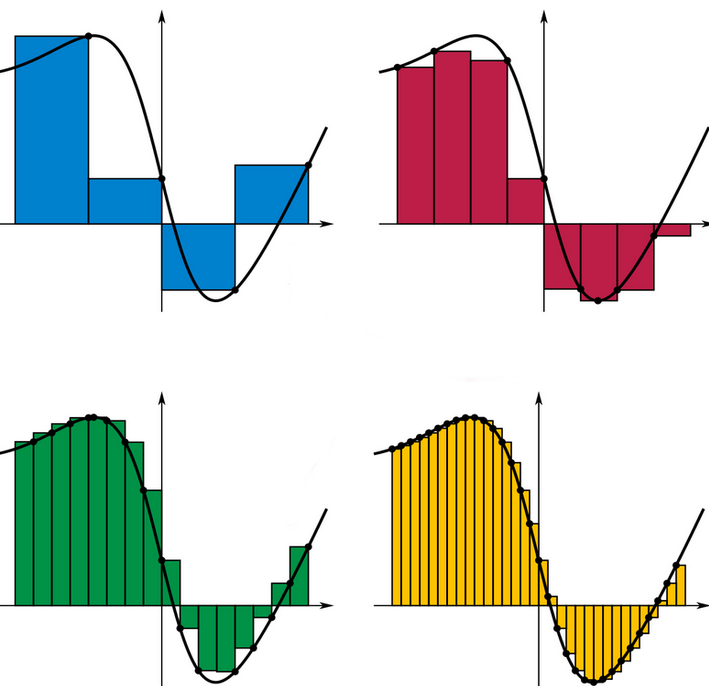
\includegraphics[scale=.3]{./diagrams/ftoc-02.png}
\end{figure}
\end{frame}

\begin{frame}
  \frametitle{Fundamental Theorem of Calculus II}
Let's assume our function is positive between $a$ and $b$, so
$f(x)\geq{}0$ for $a\leq{}x\leq{}b$. Let $F$ be an antiderivative of
$f$. Here is the \alert{mean value theorem}, a theorem we need to
assume without proof: between two arguments $r$ and $s$ we can always
find a point $q$ such that the slope of the secant line between $F(r)$
and $F(s)$ equals the slope of the tangent line at $F(q)$, so
\begin{equation}
  \label{eq:zahrahsi}
  F'(q)=\frac{F(s)-F(r)}{s-r}\mbox{ (MVT)}\notag
\end{equation}
\begin{figure}[h]
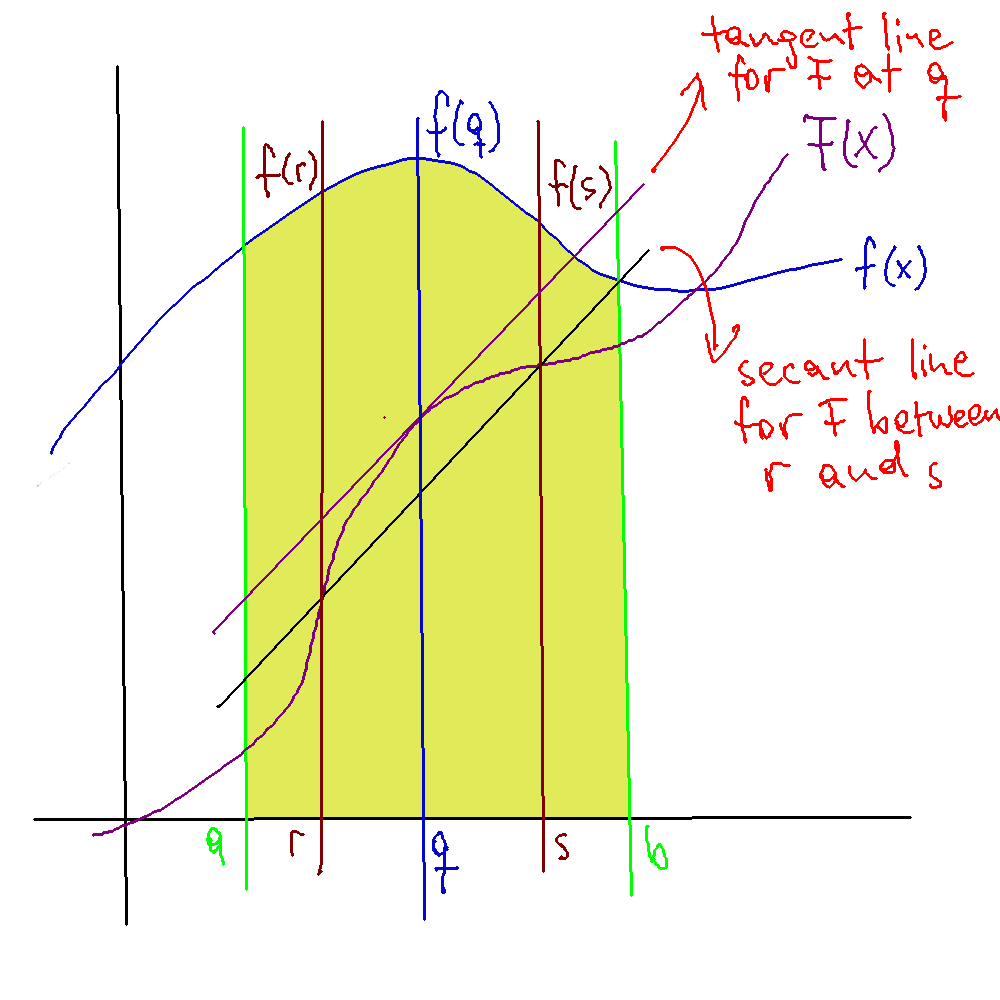
\includegraphics[scale=.13]{./diagrams/ftoc-01.png}
\end{figure}
\end{frame}

\begin{frame}
  \frametitle{Fundamental Theorem of Calculus III}
Now divide the interval from $a$ to $b$ (the notation for this
interval is $[a,b]$) into $n$ intervals that are of equal length. For
this, we need intermediate points
$a=x_{0},x_{1},x_{2},\ldots,x_{n-1},x_{n}=b$. The approximate area
under the curve between $a$ and $b$ is
\begin{equation}
  \label{eq:eikaidei}
  A\approx\frac{x_{1}-a}{n}f(x_{1}^{*})+\frac{x_{2}-x_{1}}{n}f(x_{2}^{*})+\ldots+\frac{b-x_{n-1}}{n}f(x_{n}^{*})
\end{equation}
where $x_{1}^{*}$ is some point in the first interval and so on.
Notice that the fractions all equal $(b-a)/n$ because the intervals
are all of equal length. Therefore
\begin{equation}
  \label{eq:pukaepha}
  A=\lim_{n\rightarrow\infty}\frac{b-a}{n}\left(f(x_{1}^{*})+\ldots+f(x_{n}^{*})\right)
\end{equation}
\end{frame}

\begin{frame}
  \frametitle{Fundamental Theorem of Calculus IV}
Now choose $x_{1}^{*}$ such that 
\begin{equation}
  \label{eq:bicochoh}
  f(x_{1}^{*})=F'(x_{1}^{*})=\frac{F(x_{1})-F(x_{0})}{x_{1}-x_{0}}
\end{equation}
and so on with $x_{2}^{*},x_{3}^{*},\ldots,x_{n}^{*}$. Then
\begin{equation}
  \label{eq:chabahxo}
  A=\lim_{n\rightarrow\infty}\frac{b-a}{n}\left(\frac{F(x_{1})-F(x_{0})}{x_{1}-x_{0}}+\ldots+\frac{F(x_{n})-F(x_{n-1})}{x_{n}-x_{n-1}}\right)
\end{equation}
Note that $x_{i}-x_{i-1}$ (where $i$ is any number between 1 and $n$)
is again just the length of the intervals $(b-a)/n$. After appropriate
simplification,
\begin{equation}
  \label{eq:ovooleek}
  A=F(b)-F(a)=\int_{a}^{b}f(x)\,dx
\end{equation}
\end{frame}

\begin{frame}
  \frametitle{Fundamental Theorem of Calculus V}
Here are two different ways to express the Fundamental Theorem of
Calculus.
\begin{block}{The Fundamental Theorem of Calculus}
  Suppose $f$ is continuous on $[a,b]$.
  \begin{enumerate}
  \item If $g(x)=\int_{a}^{x}f(t)\,dt$, then $g'(x)=f(x)$.
  \item $\int_{a}^{b}f(x)\,dx=F(b)-F(a)$, where $F$ is any
    antiderivative of $f$, that is, $F'=f$.
  \end{enumerate}
\end{block}
Note that we need not require $a\leq{}b$. If the limits of integration
are unintuitively placed, you can rectify the situation by using 
\begin{equation}
  \label{eq:vichujai}
  \int_{b}^{a}f(x)\,dx=F(a)-F(b)=-(F(b)-F(a))=-\int_{a}^{b}f(x)\,dx\notag
\end{equation}
\end{frame}

\begin{frame}
  \frametitle{Fundamental Theorem of Calculus Exercises}
{\ubung} Find the area under the parabola
\begin{equation}
  \label{eq:veigheph}
  y=x^{2}
\end{equation}
from $0$ to $1$.

\bigskip

{\ubung} Find the area under the cosine curve from $0$ to $b$, where $0\leq{}b\leq\frac{\pi}{2}$.
\end{frame}

\begin{frame}
  \frametitle{Other Applications: Distance and Velocity} 
  \beispiel{Distance Problem} Find the distance traveled by an object
  during a certain time period if the velocity of the object is known
  at all times. If the velocity remains constant, then the distance
  problem is easy to solve by means of the formula distance
  \begin{equation}
    \label{eq:iofaepha}
    \mbox{distance}=\mbox{velocity}\times\mbox{time}
  \end{equation}
  But if the velocity varies, it's not so easy to find the
  distance traveled. Suppose the odometer on our car is broken and
  we want to estimate the distance driven over a 30-second time
  interval. We take speedometer readings every five seconds and record
  them in the following table.

\medskip

  \begin{tabular}{|l|r|r|r|r|r|r|r|r|}\hline
    Time (s) & 0 & 5 & 10 & 15 & 20 & 25 & 30 \\ \hline 
    Velocity (ft/s) & 25 & 31 & 35 & 43 & 47 & 45 & 41 \\ \hline
  \end{tabular}
\end{frame}

\begin{frame}
  \frametitle{Other Applications: Distance}
  \begin{tabular}{|l|r|r|r|r|r|r|r|r|}\hline
    Time (s) & 0 & 5 & 10 & 15 & 20 & 25 & 30 \\ \hline 
    Velocity (ft/s) & 25 & 31 & 35 & 43 & 47 & 45 & 41 \\ \hline
  \end{tabular}

\medskip

\begin{figure}[h]
  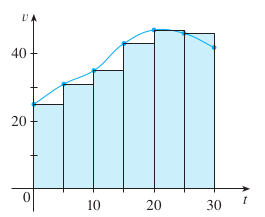
\includegraphics[scale=0.65]{./diagrams/intvel.png}
\end{figure}
\end{frame}

\begin{frame}
  \frametitle{Other Applications: Net Change Theorem}
  \begin{block}{Net Change Theorem}
    The integral of a rate of change is the net change:
    \begin{equation}
      \label{eq:booghuey}
      \int_{a}^{b}F'(x)\,dx=F(b)-F(a)
    \end{equation}
  \end{block}
\end{frame}

\begin{frame}
  \frametitle{Other Applications: Net Change Theorem}
\beispiel{Water} If $V(t)$ is the volume of water in a reservoir at
time $t$, then its derivative $V'(t)$ is the rate at which water flows
into the reservoir at time $t$. So
\begin{equation}
  \label{eq:xusicahk}
  \int_{t_{1}}^{t_{2}}V'(t)\,dt=V(t_{2})-V(t_{1})
\end{equation}
is the change in the amount of water in the reservoir between time
$t_{1}$ and $t_{2}$.

\bigskip

\beispiel{Production Cost} If $C(x)$ is the cost of producing $x$ units of
a commodity, then the marginal cost is the derivative $C'(x)$. So 
\begin{equation}
  \label{eq:quaechea}
  \int_{x_{1}}^{x_{2}}C'(x)\,dx=C(x_{2})-C(x_{1})
\end{equation}
is the increase in cost when production is increased from $x_{1}$ units to
$x_{2}$ units.
\end{frame}

\begin{frame}
  \frametitle{Net Change Theorem Exercise}
  {\ubung} Water flows from the bottom of a storage tank at a
  rate of 
  \begin{equation}
    \label{eq:iigahdae}
    r(t)=200-4t
  \end{equation}
  litres per minute, where $0\leq{}t\leq{}50$. Find the amount of
  water that flows from the tank during the first $10$ minutes.
\end{frame}

\begin{frame}
  \frametitle{End of Lesson}
Next Lesson: Area and Volume
\end{frame}

\end{document}

